\chapter{Results}\label{chapter_sta}
In preceding chapters, I have discussed a number of phenomena which provide the motivation for my exploratory study investigating the possibility of recurrent behaviors discovery from software artifacts, reviewed the relevant previous work from the research field of software repository mining, identifying unexplored and under-explored directions, and proposed a novel generic temporal data-mining technique called \mbox{SAX-VSM}, which, potentially, can automate the discovery of recurrent behaviors from software artifact measurements.

In this chapter, I shall present, evaluate, and discuss \mbox{SAX-VSM}-based implementation of the Software Trajectory Analysis framework (STA) that provides an end-to-end generic and customizable solution for the problem of recurrent behaviors discovery from software trajectories.  As I shall show, throughout my exploratory study STA has evolved from a narrow focused tool to a universal framework that facilitates software artifacts collection, their measurements, software trajectories construction, and, the most importantly, enables the recurrent behaviors discovery.

\section{Software Trajectory Analysis system overview}\label{section_sta_overview}
Before presenting and discussing the current STA implementation, I shall briefly review its background starting with the software trajectory definition. 

Recall, that the \textit{software trajectory} is defined as an abstract representation of the software product and/or process evolution by a series of temporally ordered measurements. In other words, it is a field-specific abstraction that technically is the time series with attached contextual meaning. Intuitively, this abstraction in Software Engineering is similar to that used in Physics, where trajectory is an approximate path that a moving object draws in a physical space, or in Mathematics, where trajectory is defined as a reduced in complexity sequence of states of a dynamic system (a Poincar\'{e}' map).

Note, since software metrics are numerous, many kinds of software trajectories describing a software product and process evolution can be constructed, including multidimensional trajectories. For example a trajectory whose points consist of two measurements -- churn (i.e. the velocity of software process) and cyclomatic complexity -- can be constructed in an attempt to assess the system's complexity evolution. Current STA implementation is unable to work with multidimensional data type. Nevertheless, it can be adopted and used for multidimensional data, as I shall discuss in the Section \ref{section_future_work} that is concerned with the future work.

Software Trajectory Analysis was proposed as a paradigm (i.e. a model) which, potentially, enables the extraction of \textit{meaningful} patterns from software trajectories \cite{citeulike:13159603}. As a particular criterion for the pattern meaningfulness, its association with recurrent behaviors is considered. 

Note, that STA was envisioned as a part of a larger, already existing system, called Hackystat \cite{citeulike:557296}, which provides an automation for sophisticated software process and product measurements. However due to a number of reasons, discussed throughout this Chapter and in particular in the Section \ref{feasibility2}, STA evolved into a stand alone tool which nevertheless can be plugged into Hackystat without any significant effort, thanks to the generality of a developed approach.

\subsection{Software Trajectory Analysis implementation}
Discussed in this thesis STA is implemented in Java and relies on a number of auxiliary libraries which aid in data collection \cite{jgit}, storage \cite{mybatis}, and analysis \cite{sax-vsm}. STA also relies on the relational database engine which aids in data indexing and software trajectories construction. 

STA does not have a single universal implementation. Currently, there exist three implementations customized for a particular case study (discussed in Sections \ref{case1}, \ref{case2}, and \ref{case3}). This is due to the interactive nature of data mining, where a number of data and problem -specific abstraction and aggregation steps need to be performed sequentially in order to extract the knowledge. Typically, a project-specific STA implementation consists of a number of executable modules that need to be run sequentially in order to collect software artifacts, transform them into measurements, and to load these into the database. Similarly there are executable modules whose purpose is to extract and to analyze software trajectories. Therefore, in the following sections I shall discuss STA at the abstract level pointing out its specificity and limitations.

\subsubsection{STA is generic}
The \mbox{SAX-VSM} algorithm on which STA relies for patterns discovery, does not require the user to specify any baseline thresholds when performing analyses. The system is capable to discover class-characteristic software trajectory patterns directly from the provided data. All discussed in this Chapter case-studies, namely the Android OS and PostgreSQL release patterns discovery,  PostgreSQL maintenance pattern discovery, and StackOverflow user pattern discovery, are built upon this feature.

In addition to the class-characteristic patterns discovery, SAX-VSM ranks discovered patterns by their class-characteristic power -- the property which I relate to interestingness and meaningfulness. The adequacy of this relation is examined in all three case studies.

As it is, STA can be applied to \textit{two or more} sets of software trajectories that represent logical classes, such as different projects, teams, developers, etc. Alternatively, software trajectory classes can be defined as those generated by the same entity but within distinct, non-overlapping time intervals. These intervals can be associated with specific processes (such as software release or Scrum spike) or other external and internal constraints. This approach is used in the Android OS and PostgreSQL case studies, where software trajectory classes are defined by using different time intervals while the software trajectory-generating entities are staying the same.

Yet another STA specificity is that it does not place any constraints on the form of a provided dataset. Specifically, by its design, it is robust to any kind of asymmetry among volumes of the input classes and unequal lengths of software trajectories within and among the classes. For example, in PostgreSQL case study, software trajectories length varied from few dozens to few hundreds of points within a class.

Finally note, that built upon the core Information Retrieval algorithm that is Vector Space Model, STA can be finely tuned in many ways in order to achieve the goal. Among other refinements are various weighting scheme (shown in the Table \ref{tbl:smart}), characteristic vector improvement through the relevance feedback \cite{salton-71}, and other tuning techniques \cite{intro_ir_Manning}.

\begin{figure}[t]
   \centering
   \includegraphics[width=145mm]{figures/STA12-schema-draft.eps}
   \caption{A schematic overview of the very first and the latest STA implementations. 
   Note STA evolution from a thin layer embedded into the larger system relying on external data assimilation and processing 
   mechanisms to the end-to-end generic solution for software artifact measurements analysis.}
   \label{fig:STA12-schema}
\end{figure}

\subsubsection{STA is a two-components system}\label{two_components}
In order to enhance the STA generality, and to reduce the overall system complexity, a decision has been made to decouple the data assimilation and the data analysis components using a relational database. This solution, shown at the right panel of Figure \ref{fig:STA12-schema}, allowed to successfully cope with a variety of data formats from numerous software process management and configuration systems since the internal STA data format stays unchanged for all upstream analyses allowing for interactive and efficient trajectory classes definition and their characteristic pattern discovery. 

While the database schema supporting this design varies from project to project accommodating specific data types, it is usually simple as it only contains few tables that store artifact measurements and entities that facilitate their partitioning, such as user and project records. As an example, consider the database schema used in the Android OS case study shown at the Figure \ref{fig:db-schema}. There, tables \texttt{change\_target} and \texttt{android\_change} contain information about source-code change events and their measurements, while other tables, namely \texttt{change\_people} and \texttt{change\_project}, allow for the efficient software trajectories construction when using a simple SQL \texttt{SELECT} query. For example the following query retrieves a software trajectory for the Android OS contributor: 
\begin{verbatim}
    SELECT sum(c.added_lines) `value`, 
    DATE_FORMAT(c.author_date, "%Y-%m-%d") `date` from OMAP.change c
    where c.author_id=174 and c.project_id=1
    AND c.author_date BETWEEN "2012-03-26" AND "2012-04-01"
    GROUP by `date` order by `date`;
\end{verbatim}

Currently, STA relies on MySQL database server \cite{mysql}, but any other relational database engine can be used since all database communications are performed through an object-relational mapper called MyBATIS \cite{mybatis} which can be re-configured independently from STA source code.

\begin{figure}[t]
   \centering
   \includegraphics[width=150mm]{figures/sta-schema.eps}
   \caption{An example of STA database schema used in the Android OS case study which targets the discovery of
   recurrent behaviors from the history of software change records. As shown, the schema can be divided into three 
   structural components where the change records and their summary measurements constitute the main table (middle).
   These are complemented by the information about the atomic changes (right). 
   The tables enumerating sub-projects and committers (left) are used for the data partitioning, i.e. software trajectories construction.}
   \label{fig:db-schema}
\end{figure}

\subsubsection{STA limitations}\label{sta_limitations}
There are two major limitations of Software Trajectory Analysis that are associated with its current implementation.

The first limitation is that the two or more classes analysis paradigm is not suitable for the study of a single trajectory or a single class of trajectories. While recently I have proposed a solution that enables the discovery of recurrent patterns from a single time series that is built upon symbolic discretization, grammatical inference, and the resulting grammar complexity analysis \cite{grammarviz2}, it is not discussed in this thesis as it is not yet evaluated.

The second limitation is that while it is asserted that the application of STA to two or more classes of software trajectories guarantees (by design) to yield a ranked lists of class-characteristic patterns, where recurrent patterns shall be ranked as the most important, \textit{it may fail to do so}. Such STA behavior is well understood and is directly linked to the specificity of the input data: if it contains patterns that are similar across classes under analysis, they are dismissed from the resulting list by the $\textbf{idf}$ component of VSM weighting schema as shown in Equation \eqref{formula:tfidf}. In addition, when working with \textit{only two} classes of trajectories, due to this phenomena STA reports only patterns that appeared in a single class, which is very conservative approach. For example, consider that a SAX word accounts for 50\% of all words in the Class 1 and has been observed only once in the Class 2: currently, in spite of the apparently high class-characteristic potential of the word, it will be discarded since its $\textbf{idf}=0$ and consequently \tfidf$=0$.

In order to handle this two-class issue, I employ a technique that is based on the re-labeling of samples and clustering, as discussed in Android OS and PostgreSQL case studies. For this, all the trajectories are re-labeled with unique names and treated with SAX-VSM at first; next, the k-means clustering procedure (where k is set to 2) is applied; finally, the clusters are labeled by the members voting and their centroids are considered as class-characteristic pattern vectors. As I shall show, this approach demonstrates a promising performance. Note, that this solution is not new and was pointed out before in a number of studies \cite{classification_centroids} \cite{salton-71} \cite{intro_ir_Manning}.

\section{STA Pilot studies}
Probably the most valuable in terms of insight gained into the problem of recurrent behaviors discovery from software artifacts were two exploratory studies conducted within the feasibility study phase of my research work. While the first study confirmed the possibility of recurrent behaviors discovery from artifact measurements, the SAX-VSM algorithm was developed and evaluated throughout the second study.

\subsection{Feasibility study 1: mining Hackystat software telemetry streams}
In order to investigate the feasibility of recurrent behaviors discovery from software process measurements, I have conducted a pilot study consisting of two experiments. The first experiment was based on the software telemetry streams discretization with SAX \cite{citeulike:2821475}, patterns extraction, and their frequency-based analysis. The second experiment was based on the association rule mining algorithm application to series of software development events.

Software telemetry is a data type data that is generated by the Hackystat \cite{citeulike:12929227}, which is an in-process software engineering measurement and analysis system. Software telemetry is collected with automation and is characterized by high consistency that enables unprecedented insight into performed processes, as I have already discussed in Section \ref{section_software_telemetry}. Effectively, by offering the efficient data collection, storage, retrieval mechanisms, and most importantly the consistent, fine-grained data, Hackystat provided an ideal testbed for the STA feasibility study.

The data used in study was collected from the development and deployment environments utilized by students participating in the Software Engineering class. The dataset represents Hackystat metrics collected during sixty days of a classroom project by eight students. 

An overview of the pilot Hackystat-based STA targeting recurrent behaviors discovery is shown at the left panel of Figure  \ref{fig:STA12-schema}. As mentioned, the first experiment was based on two analytical techniques: the discretization of time-series with SAX, that effectively translates real-valued telemetry streams into strings, and the occurrence frequency (i.e. support) -based discovery of recurrent patterns that is similar to that formalized and discussed later by Lin et al. in \cite{citeulike:10525778}. 

As I have shown in \cite{csdl2-10-09} this approach demonstrated the feasibility of recurrent behaviors discovery by mining of frequently occurring symbolic patterns, i.e. time series motifs \cite{sax}. Consider an example of recurrent behaviors discovery shown at the Figure \ref{fig:STA1-results}, where software trajectories built of development effort measurements shown at the left and their clustering based on the Euclidean distance between vectors of symbolic patterns occurrence frequencies shown at the right. Clearly, the hierarchical clustering process partitioned the set of trajectories separating two developers (\#2 and \#7) from the rest. Further investigation of the data revealed that these two developers demonstrated the most consistent development behavior (when discretized by 4 days window) as they spent considerable amounts of time working on the project almost daily whereas the rest of the study participants did not. Thus, the results of STA analysis were found consistent with the ground truth.

\begin{figure}[t]
   \centering
   \includegraphics[width=145mm]{figures/STA1.eps}
   \caption{Results of the pilot STA study. 
   The left panel shows eight software trajectories that are Hackystat telemetry streams 
   corresponding to development effort \cite{citeulike:557296} collected from eight developers in the course of two months.
   The right panel shows a hierarchical clustering of developers by the comparison of trajectory-corresponding sets of 
   recurrent patterns discovered with SAX discretization \cite{sax}. 
   Note two distinct groups discovered by clustering: the one that contains consistent trajectories (developers \#2 and \#7) 
   and the one with less consistent trajectories.}
   \label{fig:STA1-results}
\end{figure}

In addition to indicating the feasibility of automated recurrent behaviors discovery through the analysis of discretized measurements, the experience with pilot system highlighted a number of issues. It was found, that the major issue threating the external validity of study, was the small scale of class-room experimentation that simply did not provide an adequate and generalizable coverage of the studied phenomena. For example, it is possible that in the above experiment some of the developers characterized by ``inconsistent behavior'' may simply had their Hackystat sensors mis-configured or malfunctioning, which is difficult to recognize automatically. The second significant issue identified through experimentation was the problem of discretization algorithm parameters selection -- they have to be defined as the input, but their proper values are non-intuitive and often difficult to guess.

The second experiment investigated the applicability of an association rule mining algorithm called Apriori \cite{citeulike:775528} to the the stream of development event records collected by Hackystat. As I have shown in \cite{citeulike:13159603}, this approach also demonstrated a satisfactory performance. However, since it is impossible to recover the development events from public software artifacts, as discussed in the Section \ref{section_understanding}, this workflow has not been used in the following STA implementations.

\subsection{Feasibility study 2: mining public software repositories} \label{feasibility2}
Following lessons learned during the pilot study and the feedback collected through its discussion \cite{csdl2-10-09}, 
the decision has been made to explore the feasibility of recurrent behaviors discovery from software trajectories constructed 
by measuring public software artifacts. The chief reason behind that decision is an attempt to increase 
the generality and significance of findings  by addressing all of the essential characteristics for empirical studies based on mining 
software artifacts proposed by Gasser et al. \cite{citeulike:13058334}:  
(1) they must reflect a real-life phenomena, 
(2) provide adequate phenomena's coverage, 
(3) examine representative levels of variance, 
(4) demonstrate an adequate level of statistical significance,
(5) provide results that are comparable across projects,
(6) be reproducible. 

Unfortunately, due to much coarser granularity and inconsistency of software trajectories constructed by measuring public software artifacts, the original approach to data analysis based on frequency of observed patterns failed, and an additional study of time series mining techniques has been conducted using 2012 MSR challenge data \cite{MSRChallenge2012} from the Android OS repository. Discovery of recurrent behaviors associated with the \textit{software release pattern} was set as the study's goal.

\subsubsection{Software release pattern}
Previously, in the software engineering literature, it has been proposed, discussed, and shown that different software development cycles, and in particular the software implementation, release, and maintenance, impose various constraints on software processes \cite{citeulike:1802027} \cite{citeulike:13374124} \cite{citeulike:13374128} \cite{citeulike:6086365}. Later, Hindle et al. in \cite{citeulike:10377366} have shown that it is possible to discover the software release pattern via partitioning of software process artifacts. The authors aggregated change summaries using STDB notation (S for source, T for test, B for build, D for documentation) and have shown that the behavior of STDB summaries changes around the software release.

\subsubsection{Software release pattern discovery with STA}
Taking in account the release pattern significance and the previous experience in its discovery through analysis of public software artifacts, I have explored the possibility of software release-characteristic recurrent behaviors discovery using STA and Android OS  data. By experimenting with a number of time series transformation, discretization, and aggregation techniques, as well as with  various distance functions and ranking schema, I found that the common in Information Retrieval (IR) toolkit called Vector Space Model  (VSM) \cite{citeulike:300428} that is based on \tfidf ranking schema and Cosine similarity, demonstrated a satisfactory performance.  Specifically, as I have shown in \cite{csdl2-11-10}, STA based on the discretization with SAX \cite{sax} and mining with VSM  \cite{citeulike:300428},was found capable to discover characteristic behaviors in pre- and post- release software trajectories  constructed out of \textit{New Lines of Code} change record measurements by following the clustering methodology discussed in the previous Chapter \ref{saxvsm_clustering}. 

Consider an example shown at the Figure \ref{fig:STA2-results} for two classes of software trajectories that reflect pre- and post- 
release dynamics in counts of \textit{New Lines of Code} in the Android OS kernel OMAP repository. The left panel of the figure shows that it is possible to cluster characteristic behaviors corresponding to different time intervals where pre- and post- release behaviors are clearly separated. The right panel shows that by using pre- and post- release clusters centroids it is also possible to build a ``software release behavior classifier'' that properly assigns the majority of test intervals collected from other (not used for training) time intervals surrounding releases. The latter validates the discovered recurrent patterns characteristic capacity and the overall correctness of approach.

\begin{figure}[t]
   \centering
   \includegraphics[width=145mm]{figures/STA2.eps}
   \caption{An example of discovery of recurrent patterns in software trajectories constructed by measuring Android OS 
   repository source code change artifacts.
   The left panel shows the hierarchical clustering of pre- and post-release temporal interval-corresponding software 
   trajectories based on the Cosine similarity applied to ranked vectors of discovered characteristic patterns.
   The right panel shows the result of a cross-validation experiment where other pre- and post-release software trajectories 
   were classified by computing their NN similarity with previously discovered patterns.}
   \label{fig:STA2-results}
\end{figure}

To combat the lack of Android software repositories internal and external connectivity and the heterogeneity of data formats -- also a common issues in the MSR field -- in this STA implementation I had followed state of the art MSR approaches for data integration \cite{citeulike:13058334} \cite{cvsanaly}. In particular, similarly to a previously developed solution called softChange \cite{german04_softchange}, STA mirrors repositories and builds its own data storage facility by using a relational database engine as it is shown at the Figure \ref{fig:sta-assimilation}.

Note, that similarly to the pilot implementation, the experience with second STA highlighted the same problem of parameters selection. Moreover, this issue became even more significant since the proposed methodology was found sensitive to parameters selection. In order to address this issue, I have explored a parameters optimization scheme and implemented a DIRECT algorithm-based approach \cite{citeulike:12563460} that aids in parameters selection -- the project that essentially led to SAX-VSM development.

\section{STA 2.0 Case studies}
STA 2.0 is the most current implementation of proposed in this dissertation framework targeting the discovery of recurrent behaviors from software trajectories. It addresses all of the previously identified weaknesses and embeds all the effective solutions found throughout my exploratory studies. 

In particular, STA 2.0 is built upon the SAX-VSM algorithm including the DIRECT-based parameters optimization schema, and has a layered design where the trajectory analysis part is decoupled from the data assimilation part by a relational database.

In the next sections I shall discuss three case studies examining the applicability and performance of STA 2.0:
\begin{itemize}
 \item The Android OS software release characteristic behaviors discovery.
 \item The PostgreSQL software maintenance and software release characteristic behaviors discovery.
 \item The StackOverflow top ranked users characteristic behaviors discovery.
\end{itemize}

\subsection{Case Study 1: Android OS software release recurrent behaviors discovery}\label{case1}
As discussed above in the Section \ref{feasibility2}, during the second pilot study I have been using a time interval fixed to one week and a specific subset of users having corporate e-mails, which, in my opinion, supposed to have followed some distinguishable software development pattern. 

While this approach is logical, and is suitable for a feasibility study, it puts unreasonably strict constraints on the input data and creates a significant internal validity threat since STA only considers and reports week-long behaviors characterizing a limited group of people, which may not characterize the performed software processes adequately. This limitation was also pointed out by the reviewers of the describing the pilot publication \cite{csdl2-11-10}.

Addressing these limitations, I have designed and performed a new experiment targeting the discovery of the Android OS software release characteristic behaviors when accounting for \textbf{all} available information.

\subsubsection{Android OS dataset}
The data for this study was collected by using STA toolkit. First, the Android OS kernel OMAP repository was mirrored in order to avoid the network latency. Next, software change records were measured by STA using the mirror and populated into a dedicated database, whose schema is shown on Figure \ref{fig:STA12-schema}. This enabled an efficient measurements indexing and instant software trajectory construction, as I have explained in the section \ref{two_components}.

Note, that while the Android OS kernel OMAP dataset contains 102'602 change records authored by 7'103 authors, only 501 users were recognized by STA as active committers. This observation indirectly supports the exploratory study hypothesis that the studied project development is likely to follow some form of software process where only ``trusted developers'' (\textit{most of them having the corporate email address}) are allowed to write changes into the repository.

\begin{figure}[t]
   \centering
   \includegraphics[width=145mm]{figures/omap_removed_lines_plot.eps}
   \caption{The dynamics of the \textit{Deleted LOC} measurements throughout Android OS kernel OMAP evolution. 
   The 12 software release dates shown by vertical lines.}
   \label{fig:OMAP_dynamics}
\end{figure}

\subsubsection{Study design}
I have used three types of measurements in this study, that is (i) \textit{New LOC}, (ii) \textit{Edited LOC}, and (iii) \textit{Deleted LOC} considering 12 major releases (Android API levels 1--14, excluding API level 6 and 7 which were the minor improvements \cite{api-levels}) indicated in the Table \ref{android_table1}. The Lines Of Code (LOC) measurements were used since they represent a programmer's raw output and has been shown to reflect the size and complexity of software system along with the productivity of programmers  \cite{citeulike:341464} \cite{citeulike:13410945} \cite{citeulike:13410947}. Since in experiments  software trajectories comprised of \textit{Deleted LOC} measurements were found as having the most class-characteristic power, this measurement dynamics throughout the project history is shown on Figure \ref{fig:OMAP_dynamics} with variable granularity. Note, that the total daily values within this data stream vary from zero to few thousands while the average activity slowly decreases.

\begin{table}[t]
\caption{Counts of pre- and post- release trajectories corresponding to the \textit{Deleted LOC} dynamics per author and time interval within Android OS kernel OMAP project.}
\label{android_table1}
\centering
\begin{small}
\begin{tabularx}{\linewidth}{l l c c X X}
\toprule
Id &Release name & API level & Date & Pre-release \textit{Deleted LOC} & Post-release \textit{Deleted LOC}\\
& & & & trajectories count & trajectories count\\
\midrule
1 & Android 1.0    & 1 & 2008-09-23    &  266 &    381\\
2 & Android 1.1    & 2 & 2009-02-09     & 302 &    342\\
3 & Android 1.5     & 3 & 2009-04-27    & 330  &   177\\
4 & Android 1.6     & 4 & 2009-09-15    & 214  &   390\\
5 & Android 2.0     & 5 & 2009-10-26    & 252  &   255\\
6 & Android 2.2     & 8 & 2010-05-20    &  292  &   368\\
7 & Android 2.3     & 9  & 2010-12-06    &  209   &  203\\
8 & Android 2.3.3   & 10 & 2011-02-09  &   364  &   274\\
9 & Android 3.0     & 11 & 2011-02-22    &  308   &  341\\
10 & Android 3.1     & 12 & 2011-05-10    &  324 &    416\\
11 & Android 3.2     & 13 & 2011-07-15   &   314 &    238\\
12 & Android 4.0     & 14 & 2011-10-18    &  186  &   194\\
\bottomrule
\end{tabularx}
\end{small}
\end{table}

For each of the release dates, the release week was determined and excluded from analyses. Intervals equal to four weeks preceding, and four weeks succeeding the release week were extracted and used in the study while named as \textit{pre-release} and \textit{post-release} intervals respectively. For each contributor that authored a change record resulted in source code lines measurements change within pre- and post- release intervals, software trajectories were constructed. The total amount of trajectories within pre- and post-release intervals in \textit{Deleted LOC} measurements is shown in the Table \ref{android_table1}. 

Similar to that in the feasibility study, I have used three random software releases in order to discover pre- and post-release class-characteristic patterns. First, in order to retain more class-characteristic patterns (addressing the limitation discussed in section \ref{sta_limitations}), trajectories labeled by two labels (pre- and post- release) were relabeled at first by assigning them to three pairs of  pre- and post- release software trajectory classes labeled as \textit{pre-1}, \textit{pre-2}, \textit{pre-3}, and \textit{post-1}, \textit{post-2}, and \textit{post-3} respectfully. At the second step, SAX-VSM was applied to these six classes and the optimal parameters set was determined with DIRECT optimization scheme (Section \ref{section-direct}). At the third step, software trajectories from each class were discretized into a bag of words with SAX using optimal parameters and \tfidf statistics was computed. Finally, the resulting weight vectors were clustered using SAX-VSM implementation of spherical k-Means clustering (Section \ref{saxvsm_clustering}) with $k$=2 and the resulting cluster centroids, corresponding to pre- and post-release clusters, were extracted. These centroids were used in the validation step as vectors comprised of class-characteristic patterns. An example of these vectors is shown in Table \ref{android_weights}.

\begin{table}[t]
\centering
\makebox[0pt][c]{\parbox{\textwidth}{%
\begin{minipage}[b]{0.47\hsize}\centering
\begin{tabular}{c c}
\toprule
\multicolumn{2}{c}{Pre-release centroid} \\
pattern & weight \\
\midrule
ebbbebbbbbbb    & 0.1748588272 \\
bbbbbcbbbebb    & 0.1083403654 \\
bbbbbbbdebbb    & 0.0901908199 \\
bbbbbbbbdebb    & 0.0901908199 \\
bbbbbbdebbbb    & 0.0901908199 \\
$\dots$ &$\dots$\\
\bottomrule
\end{tabular}
\end{minipage}
    \hfill
\begin{minipage}[b]{0.47\hsize}\centering
\begin{tabular}{c c}
\toprule
\multicolumn{2}{c}{Post-release centroid} \\
pattern & weight \\
\midrule
edbbbbbbbbbb   & 0.1995655982\\
bbbbbebbcbbb   & 0.1533399084\\
bbbbbbebbcbb   & 0.1533399084\\
bbbbbbbebbcb   & 0.1533399084\\
bbbbbbbbebbc    & 0.1533399084\\
$\dots$&$\dots$\\
\bottomrule
\end{tabular}
\end{minipage}%
\caption{An excerpt from pre- and post-release class-characteristic pattern vectors obtained by mining the \textit{Deleted LOC} trajectories in Android OS case study. The total size of each vector is 622 weighted patterns.}
\label{android_weights}
}}
\end{table}

The class-characteristic vectors computed at previous step were evaluated for class-characteristic power using cross validation. For this, a SAX-VSM classifier was constructed and its accuracy was determined by classifying pre- and post- release trajectories corresponding to all software releases under analysis.

\subsubsection{Results}
The outlined above procedure was applied to 4 random samples each of which consists of 3 releases (\textit{Train releases} in Table  \ref{android_accuracy}) using three types of software trajectories (\textit{Software metric} in Table  \ref{android_accuracy}). The accuracy of resulting classifiers is shown in the Table  \ref{android_accuracy}. As shown, the best performing classifier was built using the intervals corresponding to the set of releases \{4,6,9\} (i.e. Android OS API Levels 4, 8, and 11) and the \textit{Deleted LOC} measurements.

\begin{table}
\begin{tabularx}{\linewidth}{l X X X l}
\toprule
Software metric & Train releases  & Parameters      & Accuracy        & Note\\
\midrule
added code lines &       1,3,5 &  18,7,12& 54.00\% & biased towards post-\\
added code lines &        4,6,9 &  15,15,5 &58.33\% & biased towards post-\\
added code lines &      5,8,11 & 12,10,10 &       66.66\% & biased towards pre-\\
added code lines &       1,6,12 & 28,5,14& 66.66\% & biased towards pre-\\
edited lines &   1,3,5  & 24,10,4& 62.50\%& biased towards post-\\
edited lines &   4,6,9  & 24,5,12& 58.33\% & biased towards post-\\
edited lines &   5,8,11&  22,7,7 & 62.50\%  &biased towards pre-\\
edited lines &   1,6,12 & 18,8,7 & 58.33\% & biased towards pre-\\
deleted lines &  1,3,5  & 24,10,4& 58.44\% & biased towards pre-\\
deleted lines &  4,6,9  & 12,12,5 &\textbf{75.00}\%  & \\
deleted lines &  5,8,11&  24,5,7 & 61.50\% & biased towards post-\\
deleted lines &  1,6,12 & 24,5,11 &62.50\% & biased towards pre-\\
\bottomrule
\end{tabularx}
\caption{Statistics for a number of software release classifiers built using the Android OS kernel OMAP data. As shown, a typical classifier for post- and pre- release behaviors based on LOC change measurements achieves an accuracy above 60\%. The best performing classifier demonstrated 75\% accuracy and was trained on using the deleted lines of code measurements corresponding to API level releases \{4,6,9\}.}
\label{android_accuracy}
\end{table}

The Table \ref{android_table3} shows details of the classification with the best performing classifier. As shown, it is slightly biased towards post-release. The first 5 class-characteristic patterns for both classes are shown in the Table \ref{android_weights}, while examples of software trajectories containing these are shown in Figure \ref{fig:OMAP_patterns}.

\afterpage{% 
\begin{table}[t!]
\centering
\makebox[0pt][c]{\parbox{\textwidth}{%
\begin{minipage}[b]{0.47\hsize}\centering
\begin{tabular}{l c c c}
\toprule
Class & pre- & post- & classification \\
& cosine & cosine & result  \\
\midrule
pre-1&   0.0112 & 0.0076 & ok\\
pre-2&   0.0073&  0.0095 & miscl.\\
pre-3&   0.0108 & 0.0083&  ok\\
pre-4 &  0.0223 & 0.0066&  ok\\
pre-5 &  0.0093& 0.0143 & miscl.\\
pre-6 &  0.0061 & 0.0143&  miscl.\\
pre-7 &  0.0083& 0.0088 & miscl.\\
pre-8&  0.0120&  0.0107&  ok\\
pre-9 &  0.0186&  0.0076 & ok\\
pre-10 & 0.0095&  0.0085 & ok\\
pre-11 & 0.0128 & 0.0088 & ok\\
pre-12 & 0.0115 & 0.0091&  ok\\
\bottomrule
\end{tabular}
\end{minipage}
    \hfill
\begin{minipage}[b]{0.47\hsize}\centering
\begin{tabular}{l c c c}
\toprule
Class & pre- & post- & classification \\
& cosine & cosine & result  \\
\midrule
post-1  &0.0088 & 0.0128 & ok\\
post-2 & 0.0098 & 0.0074 & miscl.\\
post-3 & 0.0056 & 0.0081 & ok\\
post-4&  0.0077 & 0.0175 & ok\\
post-5 & 0.0049 & 0.0058 & ok\\
post-6 & 0.0055 & 0.0144 & ok\\
post-7 & 0.0083 & 0.0100 & ok\\
post-8 & 0.0100 & 0.0104 & ok\\
post-9 & 0.0189 & 0.0068 & miscl.\\
post-10& 0.0116& 0.0128& ok\\
post-11& 0.0087 & 0.0103&  ok\\
post-12& 0.0071 & 0.0072&  ok\\
\bottomrule
\end{tabular}
\end{minipage}%
\caption{The classification results for Andriod OS release classifier. Higher cosine value corresponds to smaller angle 
and is better. Overall, this classifier demonstrated an accuracy of 75\%.}
\label{android_table3}
}}
\end{table}
\begin{figure}[h!]
   \centering
   \includegraphics[width=150mm]{figures/omap_deleted_lines_patterns_plot.eps}
   \caption{Examples of software trajectories representing the dynamics of \textit{Deleted LOC} measurements throughout Android OS kernel OMAP evolution which contain the best and second best class-characteristic patterns.}
   \label{fig:OMAP_patterns}
\end{figure}
} % end of argument of `\afterpage` command

\subsubsection{Discussion}
Quite intriguing and unexpected, the best pre- and post-release class-characteristic patterns were discovered in software trajectories comprised of the \textit{Deleted LOC} measurements. These were found using the discretization parameters of sliding window 12, PAA 12, and alphabet of the size 5, i.e. by converting normalized daily measurement into a letter taken from an alphabet of the size 5. 

The patterns shown at the Figure \ref{fig:OMAP_patterns} reveal that the best class-characteristic behavior for pre-release class when accounting to the \textit{Deleted LOC} measurements is to perform two deletions of approximately equal volume separated by three days and followed by a week of inactivity, whereas the best class-characteristic behavior for the post-release class is to perform decreasing in volume deletions during two consecutive days followed by 10 days of inactivity. Second best class-characteristic patterns were also found to follow a similar pattern -- different in volume source code lines deletion events separated/followed by a time interval.

Overall, the discovered patterns are impossible to translate into a sensible description without the discussion with developers. Unfortunately, despite of my effort, I was not able to communicate with key contributors from Android OS kernel OMAP team. 

Through my own investigation of commit messages and source code files corresponding to deletion events of the best pre-release patterns, I have found that majority of them correspond to a normal software development cycle where the changes were staged, reviewed, and signed off by the project managers. What was interesting however, is that many of the deletion events were reflecting the code clean-up from Linux artifacts (Android OS is based on the Linux kernel), such as SCSI modules, or other platform hardware-related code, therefore, since observed among many trajectories, they may reflect a systematic Android OS release-related activities.

\clearpage

\subsection{Case Study 2: PostgreSQL software maintenance and software release recurrent behaviors discovery}\label{case2}
Similar to the previous case study, I have explored the possibility of recurrent behaviors discovery from software trajectories that were constructed by measuring software change artifacts from PostgreSQL public software repository. 
 
PostgreSQL is an open-source database developed by the PostgreSQL Global Development Group consisting of a number of volunteers employed and supervised by companies such as Red Hat and EnterpriseDB \cite{postgre-contrib}. It has a large number of extensions written by contributors and is available for many platforms including Linux, FreeBSD, Solaris, Microsoft Windows and Mac OS X.

One of the particular characteristics of PostgreSQL software development process is its regular CommitFest events \cite{commit-fest}. As PostgreSQL team explains it, a CommitFest (CF) event is a ``\textit{periodic break to PostgreSQL development that focuses on patch review and commit rather than new development}'' -- a description that allows to classify it as a \textit{maintenance activity} whose purpose is to promptly review and to respond with a feedback to development community without waiting for a major release. Contributors are encouraged by the core development team to submit patches into the development mailing list. Within a CF event, these patches are reviewed, tested, and the decision for a final review and commit is made.  Typically, CFs tend to run for one month with a one month gap between them, however, when the core team is busy with a PostgreSQL major release, there may be several months without CF events followed by a ReviewFest (RF), which helps to pre-organize patches, and a CF . 

Up to the data retrieval date, 18 CF events were held. Typically, after reviewing and testing of a patch submitted for CF, developers assign it to one of the categories: ``Needs Review'', ``Ready for Commit'', ``Committed'', ``Returned with Feedback'', or ``Rejected''. While the very first CF event dealt with 66 patches, from which 37 were committed, the latest CF event dealt with 108 patches in the review queue out of which 7 were marked for additional review, 14 as ready to commit, 36 were committed, and 42 were returned with a feedback.

\begin{figure}[t!]
   \centering
   \includegraphics[width=150mm]{figures/postgre_commits_dynamics.eps}
   \caption{PostgreSQL evolution. The top panel shows dynamics of the weekly commits into PostgreSQL repository, the middle panel shows \textit{Churn}, and the bottom panel shows \textit{Added LOC} measurements dynamics throughout the analyzed Commit Fest events. Dotted vertical lines show the release dates.}
   \label{fig:postgre_dynamics}
\end{figure}

\subsubsection{PostgreSQL dataset}
Similar to Android OS study, the PostgreSQL data was collected by using STA data assimilation toolkit and stored in the same database. The dataset consists of 35'890 change records authored by 38 authors. The overall commit activity shown at the top panel of Figure \ref{fig:postgre_dynamics} indicates that the project has been active throughout the years. The middle and bottom panels of the Figure \ref{fig:postgre_dynamics} show \textit{Churn} and \textit{Added LOC} aggregated software trajectories and Commit Fest events.

\subsubsection{Study design}
Based on the PostgreSQL development team documentation of their software maintenance process called Commit Fest \cite{commit-fest}, the main goal of this study  was to discover Commit Fest -characteristic recurrent behaviors. The secondary goal was to explore the software release pattern for 19 PostgreSQL releases from 6.0 dated by 1997-01-29 to 9.2 dated by 2012-09-10. The releases are shown at the Figure \ref{fig:postgre_dynamics}.

\begin{table}[t!]
\centering
\makebox[0pt][c]{\parbox{\textwidth}{%
\begin{minipage}[b]{0.47\hsize}\centering
\begin{tabular}{lcc}
\multicolumn{3}{l}\large{Commit Fest behaviors experiment\qquad}\\
\toprule
Trajectory & Discretization & LOOCV \\
class & parameters & accuracy \\
\midrule
added LOC     &  6,5,8  & 72.22\% \\
edited LOC    &  14,5,5 & \textbf{75.00}\% \\
deleted LOC   &  8,6,10 & \textbf{75.00}\% \\
added files    & 12,8,5 & 65.71\% \\
edited files   & 12,4,11& 66.67\% \\
deleted files &  27,7,3 & 55.17\% \\
\bottomrule
\end{tabular}
\end{minipage}
    \hfill
\begin{minipage}[b]{0.47\hsize}\centering
\begin{tabular}{lcc }
\multicolumn{3}{l}\large{Software Release behaviors experiment\qquad}\\
\toprule
Trajectory & Discretization & LOOCV \\
class & parameters & accuracy \\
\midrule
added LOC  &     14,5,7&  \textbf{80.56}\% \\
edited LOC  &    5,5,14 & 75.00\% \\
deleted LOC  &   10,5,11& 72.22\% \\
added files   &  16,4,10& 64.71\% \\
edited files  &  6,4,7 &  \textbf{80.56}\% \\
deleted files  & 18,5,12& 56.25\% \\
\bottomrule
\end{tabular}
\end{minipage}%
\caption{The Leave One Out Cross Validation results for PostgreSQL aggregated trajectories. The discretization parameters are ordered as the sequence of sliding window size, PAA size, Alphabet size.}
\label{postgre_table1}
}}
\end{table}

In this study, since the average activity of individual contributors is quite sparse, I have used aggregated software trajectories which were constructed by measuring \textit{all} change records without differentiating them by committers or authors. These aggregated trajectories, in turn, were cut into the pieces representing CF and non-CF software trajectories using stipulated in \cite{commit-fest} dates. For example, for \textit{Added LOC} measurements, a single software trajectory was constructed at first, then, its continuous intervals within Commit Fest intervals were extracted and labeled as CF-corresponding software trajectories, whereas the rest of continuous intervals was labeled as non-CF software trajectories. The pre- and post-release software trajectory classes were constructed in the similar fashion but by using four weeks preceding and four weeks succeeding the release week.

\begin{figure}[t]
   \centering
   \includegraphics[width=150mm]{postgre_cf_patterns.ps}
   \caption{Examples of class-characteristic behaviors discovered with SAX-VSM in PostgreSQL Commit Fest experiments. Note, that the large commits surrounded by no-activity intervals are characteristic to the regular development, whereas smaller in the volume, frequent commits are characteristic to the Commit Fest -corresponding development intervals. }
   \label{fig:postgre_cf_patterns}   
   \includegraphics[width=145mm]{figures/postgre_release_patterns.ps}
   \caption{Examples of class-characteristic behaviors discovered with SAX-VSM in PostgreSQL Software Release experiments. Note, that relatively large commits followed by low activity are characteristic for pre-release intervals, whereas post-release development is characterized by frequent commits.}
   \label{fig:postgre_release_patterns}
\end{figure}

Overall there were 18 software trajectories constructed for Commit Fest class and 18 for non-Commit Fest class, whose length varied in a range from 27 to 183. In addition, 19 software trajectories for pre-Release and 19 software trajectories for post-Release were constructed, each of them spanning 28 days (i.e. four weeks). Note, that the difference in trajectories length does not affect STA performance as it was shown in the Section \ref{saxvsm_robustness}.

For both, PostgreSQL Commit Fest and PostgreSQL Software Release experiments, a common Leave One Out Cross Validation (LOOCV) \cite{citeulike:11275990} evaluation was performed in order to estimate how accurately an STA-discovered predictive model (that is a VSM classifier based on the class-characteristic vectors) would perform in practice.

\subsubsection{Results}
The results of LOOCV experiments are shown in the Table \ref{postgre_table1}. Overall, similar to the Android OS study, it was found that a resulting characteristic-pattern based classifier performs with an accuracy above 60\%. The best accuracy was achieved by using \textit{Edited LOC} and \textit{Deleted LOC} trajectories for Commit Fest study, whereas patterns from \textit{Added LOC} and \textit{Edited Files} software trajectories characterized the Software Release the best. The Figures \ref{fig:postgre_cf_patterns} and \ref{fig:postgre_release_patterns} show examples of patterns from both studies.

\subsubsection{Discussion}
First of all, note that in the PostgreSQL study, a typical classifier built upon class-characteristic behaviors discovered with STA achieved a comparable accuracy with that of Android OS study, while the best classifiers outperformed that of Android OS. Although  this can be explained by differences in the experimental design (random training sample in Android OS and LOOCV in PostgreSQL), alternatively, the better result can be explained by a nature of used software trajectories -- individual (Android OS) versus aggregated (PostgreSQL).

Second, note that in contrast to the Android OS study, class-characteristic behaviors discovered in PostgreSQL study are easier to comprehend visually and to interpret. Both, the non-Commit Fest and pre-Software Release patterns are characterized by stretches of low activity interrupted by large in volume commits (the team focuses on the release and new development), whereas Commit Fest and post-Software Release trajectories are characterized by stretches of frequent, but moderate activity (team performs maintenance) -- both findings are in accord with PostgreSQL process description \cite{commit-fest}.
\clearpage

\subsection{Case Study 3: mining user-characteristic behaviors in Stack Overflow data}\label{case3}
Stack Overflow (SO) is a question and answer website created in 2008 that is primarily used by computer programmers. There, users are actively encouraged to participate in the community by creating public user profiles and engaging into discussions by asking good questions and providing relevant answers. As a form of gamification, this desirable user behavior is rewarded with a combination of a numerical score called reputation, and ``badges'' that implement a goals framework. 

The reputation points are awarded when individual activities are performed, such as asking a good question, providing a good answer, or commenting. There is a hierarchy of badges, from the lowest ``bronze badges'', that are relatively common and easy to achieve, to ``golden badges'', that are awarded for long term dedication and recognition from the community. Overall, the reputation and badges are an estimate of how much the community trusts the user and how much valuable contribution she has provided. Naturally, these incentives lead users to attempt to achieve as much reputation and as many badges as possible to demonstrate their expertise and to gain respect in the community. Some of these badges can be awarded recurrently, which likely to explain how user \#22656, Jon Skeet, collected over 11'000 of these as per time of writing.

Several goals were set for this study. The first goal was to explore the STA applicability to the problem of discovery of characteristic recurrent behaviors from daily and weekly user activity patterns. The second goal was to explore the applicability of a popular bioinformatics tool called WebLogo \cite{weblogo}, that creates graphical representations (logos) revealing significant patterns from a multiple sequence alignment. Since STA discovers recurrent patterns in the symbolic space, I have hypothesized that WebLogo figures shall allow summarizing numerous discovered patterns for visual comprehension. The third goal was to explore differences among the top SO users daily and weekly activity patterns in order to gain an insight into their productivity. 

\subsubsection{StackOverflow data}
The data used in this study was obtained from the Stack Overflow public release dump that is dated by August 2012 and contains over four years of the website content evolution. The dataset contains information about the users, their comments, posts, and related activities, a subset of voting history, and records about awarded badges.  Overall, the dataset accounts for 1.3M of users which created 10.4M of posts (3.5M of questions, 6.9M of answers), and 14M of comments. In addition, there is information about 28M of votes. The weekly dynamics of new Questions, Answers, and newly registered users is shown at the Figure \ref{fig:stack_dynamics}.

For the experimentation I have selected 5 top users whose summary is shown in the Table \ref{so_table}. Note, that the top three users were active for the almost whole time span considered in this study.

\begin{figure}
\centering

\includegraphics[width=150mm]{stack_overview.eps}
\caption{Stack Overflow weekly dynamics overview. Left panel shows the evolution of Questions and Answers, whereas the right panel shows the curve of new users registration.}
\label{fig:stack_dynamics}   
\end{figure}

\begin{table}[]
\begin{small}
\begin{tabularx}{\linewidth}{l X c c c c c c}
\toprule
User   & Reputation   &   Answer & \multicolumn{2}{c}{Daily  trajectories} & & \multicolumn{2}{c}{Weekly trajectories}\\
& & acceptance rate & \multicolumn{2}{c}{before \& after weighting} & & \multicolumn{2}{c}{before \& after weighting}\\
\midrule
Jon Skeet   & 465166 & 60\% &1401 & 318 & \qquad & 199 & 113 \\
Darin Dimitrov   &  343191 & 59\% & 1270  & 347 & &192 & 168\\
Marc Gravell & 325797 & 52\%  &1384 &525 & &197 & 153 \\
BalusC  & 298811 & 66\% &1002 &329 & &142 & 83 \\
Hans Passant & 271982 & 59\% &1165    &355 & &177 & 148\\
\bottomrule
\end{tabularx}
\caption{Descriptive statistics for StackOverflow users with highest reputation.}
\label{so_table}
\end{small}
\end{table}

\subsubsection{Study design}
In order to explore recurrent behaviors of five top StackOverflow users with STA, I have constructed software trajectories by summarizing amounts of user-created questions, answers, and comments per hour and per day. These were used to construct the daily and weekly activity trajectories. Next, each daily trajectory was discretized into a 8-letters string with SAX (i.e. by aggregating values for consecutive 3 hours) while each weekly trajectory was discretized into 7 letters string (a letter per day). For both discretization procedures I have used an alphabet of the size 3 whose letters $(A,B,C)$ can be interpreted as (``\textit{low}'', ``\textit{medium}'', and ``\textit{high}'') activity levels. The intuition behind this ABC-coding schema is that it shall help to reveal the differences in users daily and weekly activity dynamics and, possibly, shed a light on the differences in their reputation score.

\begin{figure}[t]
   \centering
   \includegraphics[width=150mm]{rugs.eps}
   \caption{A comparison of the activity pattern visualization techniques. Figures at left convey the most information by accounting for each hour and day, showing J. Skeet's increasing involvement over time. Plots at the middle convey the minimal amount of information by showing averaged summaries. Plots at right are made with WebLogo \cite{weblogo} using discretized with ABC-notation trajectories -- these compactly convey the information about daily/weekly behaviors variance and frequency by the letter height; the longitudinal aspect is lost, however.}
   \label{fig:rugs}   
\end{figure}

Within my dissertation proposal, and in the following work \cite{csdl2-10-09}, I have discussed the possible use of Bioinformatics tools for the discovery and visualization of patterns extracted from discretized software trajectories. In this exploratory study, I have utilized a widely known visualization tool called WebLogo \cite{weblogo} that creates graphical representation of patterns found within a multiple sequence alignment. As pointed out by the authors, ``\dots \textit{sequence logos provide a precise description of sequences similarity and can rapidly reveal significant features of the alignment otherwise difficult to perceive}''. Each logo generated by the tool consists of stacked letters, one stack for each position in the sequence. The overall height of each column indicates the sequence conservation at that position, while the height of symbols within the column reflects the relative frequency of the corresponding letter at that position.

The Figure \ref{fig:rugs} shows a comparison of WebLogo figures with two other visualization techniques conveying the same information about Jon Skeet's behaviors: the rug plot, and the averaged curve. As shown, the logo provides less resolution than a rug plot, but much more than a curve, which makes it an acceptable visualization tool when accounting for internal symbolic information representation within STA. While WebLogo allows the user to specify palette of colors for each letter, in this study I have used the two colors scheme for simplicity and in order to contrast high intensity intervals. 

\begin{figure}[t]
   \centering
   \includegraphics[width=145mm]{Stack-Summary.eps}
   \caption{WebLogo figures for top SO users representing their daily behaviors. Here, letters (\textit{A,B,C}) corresponds to (\textit{low,medium,} and \textit{high}) levels of activity. Note, that SAX-VSM pattern ranking process changed the effort distribution. 
   The recurrent behaviors shown at logos were partially confirmed by respective SO users. 
   The excluded behaviors represent a very common behavioral pattern \cite{activity_patterns}: 
   the increasing activity levels from 9AM to 3PM and the decreasing activity levels from 3PM to 12AM.}
   \label{fig:stack_daily}   
\end{figure}

\subsubsection{Results}
The results of STA and WebLogo application to StackOverflow data are shown at the Figure \ref{fig:stack_daily} for daily patterns and at the Figure \ref{fig:stack_weekly} for weekly patterns. At each figure I also compare the WebLogo-created logos for user-characteristic behaviors before and after applying SAX-VSM ranking. Note, that the ranking changes not only the amount of observed patterns (Table \ref{so_table}) but the activity levels distribution by excluding common patterns and ranking.

\begin{figure}[t]
   \centering
   \includegraphics[width=145mm]{Stack-Summary-Weekly.eps}
   \caption{WebLogo figures for top SO users representing their daily behaviors. Here, letters (\textit{A,B,C}) corresponds to (\textit{low,medium,} and \textit{high}) levels of activity. Note, that SAX-VSM pattern ranking process changed the effort distribution. 
   The excluded behaviors are likely to represent a very common behavioral pattern: peaking at the mid-week performance and work-free weekends.}
   \label{fig:stack_weekly}   
\end{figure}

The analysis of logo images for daily behaviors reveals that there are significant differences in the characteristic behavior patterns among the top SO users. For example, Jon Skeet's logo shows that his activity peaks in intervals (6AM - 9AM) and (3PM-9PM), which is confirmed by his public comment \cite{skeet}: ``\textit{\dots I have a longish commute both ways each day: a 3G data dongle lets me answer questions during that time. I spend a fair amount of time in the evening on my computer for whatever reason (coding, writing talks or articles, etc) - I pop onto SO every so often. While at work, I tend to check SO while I have tests running, a deploy, or a build \dots}". Through personal communication I was also able to confirm the characteristic daily behavior of Marc Gravell, whose daily routines are structured by commute and other constraints, whereas Darin Dimitrov pointed out that his activity at SO are not structured in any way, which may explain that his logo images are more difficult to interpret (especially early morning (1AM-3AM) ``C''s and considerably high weekend activity) and that the vector of his ranked behaviors was clustered separately of that with Skeet and Gravell as shown at the Figure \ref{fig:stack_clusters}.

\begin{figure}[t]
   \centering
   \includegraphics[width=145mm]{so_clusters.eps}
   \caption{Clustering of SO users by STA. Note that D.Dimitrov's characteristic behaviors were found very different from those of J. Skeet, while their overall reputation scores are next to each other.}
   \label{fig:stack_clusters}   
\end{figure}

\subsubsection{Discussion}
While STA was able to discover user-characteristic patterns and WebLogo produced easily interpretable figures, clearly, these do not provide a sufficient knowledge why Jon Skeet's reputation is so high -- in the daily behaviors study (3 green ``C'' at the top) and in the weekly behaviors study (4 green ``C'' at the top) his activity patterns were at the level with those of other users. It is hard to conclude it better than Jon's own comment \cite{skeet}: ``\textit{\dots Often two answers may look quite similar, but one just about has an edge on the other - either it's explained just that bit better, or has one more piece of information, or a code sample. I'd like to hope that I have that sort of edge, and that that's why my answer would get more votes in that situation. But hey, I could easily be wrong! \dots}". Also, Skeet's habit of engaging into StackOverflow activities while en route is consistent with previously reported (non-scientific) observations concerning the impact of daily routines on productivity \cite{tharp_habit}.

It was found that WebLogo provides a very efficient and reasonably effective way to convey the discretized trajectories summary, however, when a long time interval is considered it may fail to reveal the longitudinal phenomena evolution when compared with the rug plot-based visualization. Yet another WebLogo shortcoming is that while providing an excellent position-wise visualization, it fails to convey full pattern frequencies, which may affect the visualization effectiveness.

Note, that excluded by STA weighting daily behaviors correspond to a typical activity pattern expected from an office worker \cite{activity_patterns}, whose activity throughout the work week increases from 9AM, peaks at noon, and gradually degrades within the rest of the day. The excluded weekly behaviors also likely to be typical for office workers.

%\begin{figure}[t]
%   \centering
%   \includegraphics[width=145mm]{ChicagoActivity.eps}
%   \caption{An illustration from \cite{activity_patterns} showing typical temporal rhythms discovered on a weekday in Chicago.}
%   \label{fig:chicago_activity}   
%\end{figure}

\epigraph{The purpose of computing is insight, not numbers.}{Richard Hamming}
